% Created by tikzDevice version 0.12.3.1 on 2021-07-09 17:48:53
% !TEX encoding = UTF-8 Unicode
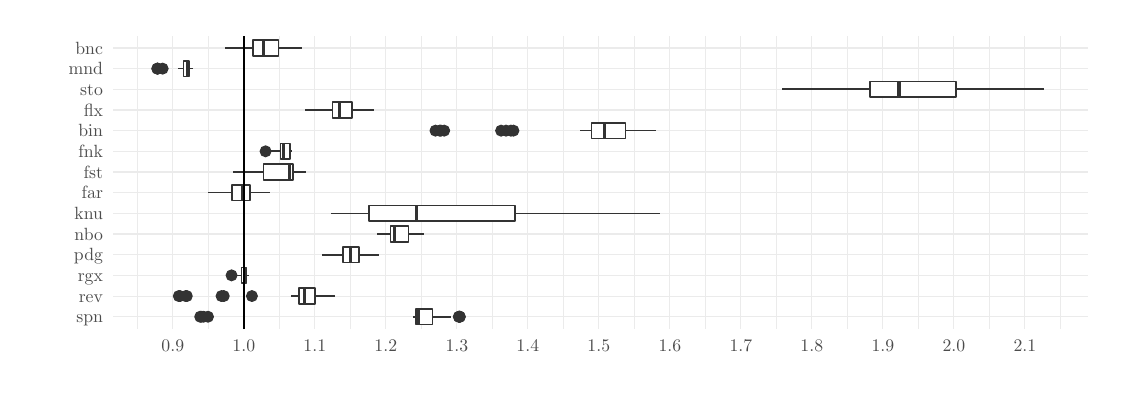
\begin{tikzpicture}[x=1pt,y=1pt]
\definecolor{fillColor}{RGB}{255,255,255}
\path[use as bounding box,fill=fillColor,fill opacity=0.00] (0,0) rectangle (390.26,130.09);
\begin{scope}
\path[clip] ( 30.80, 21.16) rectangle (383.14,127.24);
\definecolor{drawColor}{gray}{0.92}

\path[draw=drawColor,line width= 0.2pt,line join=round] ( 39.61, 21.16) --
	( 39.61,127.24);

\path[draw=drawColor,line width= 0.2pt,line join=round] ( 65.27, 21.16) --
	( 65.27,127.24);

\path[draw=drawColor,line width= 0.2pt,line join=round] ( 90.93, 21.16) --
	( 90.93,127.24);

\path[draw=drawColor,line width= 0.2pt,line join=round] (116.58, 21.16) --
	(116.58,127.24);

\path[draw=drawColor,line width= 0.2pt,line join=round] (142.24, 21.16) --
	(142.24,127.24);

\path[draw=drawColor,line width= 0.2pt,line join=round] (167.90, 21.16) --
	(167.90,127.24);

\path[draw=drawColor,line width= 0.2pt,line join=round] (193.55, 21.16) --
	(193.55,127.24);

\path[draw=drawColor,line width= 0.2pt,line join=round] (219.21, 21.16) --
	(219.21,127.24);

\path[draw=drawColor,line width= 0.2pt,line join=round] (244.87, 21.16) --
	(244.87,127.24);

\path[draw=drawColor,line width= 0.2pt,line join=round] (270.52, 21.16) --
	(270.52,127.24);

\path[draw=drawColor,line width= 0.2pt,line join=round] (296.18, 21.16) --
	(296.18,127.24);

\path[draw=drawColor,line width= 0.2pt,line join=round] (321.84, 21.16) --
	(321.84,127.24);

\path[draw=drawColor,line width= 0.2pt,line join=round] (347.50, 21.16) --
	(347.50,127.24);

\path[draw=drawColor,line width= 0.2pt,line join=round] (373.15, 21.16) --
	(373.15,127.24);

\path[draw=drawColor,line width= 0.4pt,line join=round] ( 30.80, 25.64) --
	(383.14, 25.64);

\path[draw=drawColor,line width= 0.4pt,line join=round] ( 30.80, 33.11) --
	(383.14, 33.11);

\path[draw=drawColor,line width= 0.4pt,line join=round] ( 30.80, 40.59) --
	(383.14, 40.59);

\path[draw=drawColor,line width= 0.4pt,line join=round] ( 30.80, 48.06) --
	(383.14, 48.06);

\path[draw=drawColor,line width= 0.4pt,line join=round] ( 30.80, 55.53) --
	(383.14, 55.53);

\path[draw=drawColor,line width= 0.4pt,line join=round] ( 30.80, 63.00) --
	(383.14, 63.00);

\path[draw=drawColor,line width= 0.4pt,line join=round] ( 30.80, 70.47) --
	(383.14, 70.47);

\path[draw=drawColor,line width= 0.4pt,line join=round] ( 30.80, 77.94) --
	(383.14, 77.94);

\path[draw=drawColor,line width= 0.4pt,line join=round] ( 30.80, 85.41) --
	(383.14, 85.41);

\path[draw=drawColor,line width= 0.4pt,line join=round] ( 30.80, 92.88) --
	(383.14, 92.88);

\path[draw=drawColor,line width= 0.4pt,line join=round] ( 30.80,100.35) --
	(383.14,100.35);

\path[draw=drawColor,line width= 0.4pt,line join=round] ( 30.80,107.82) --
	(383.14,107.82);

\path[draw=drawColor,line width= 0.4pt,line join=round] ( 30.80,115.29) --
	(383.14,115.29);

\path[draw=drawColor,line width= 0.4pt,line join=round] ( 30.80,122.76) --
	(383.14,122.76);

\path[draw=drawColor,line width= 0.4pt,line join=round] ( 52.44, 21.16) --
	( 52.44,127.24);

\path[draw=drawColor,line width= 0.4pt,line join=round] ( 78.10, 21.16) --
	( 78.10,127.24);

\path[draw=drawColor,line width= 0.4pt,line join=round] (103.75, 21.16) --
	(103.75,127.24);

\path[draw=drawColor,line width= 0.4pt,line join=round] (129.41, 21.16) --
	(129.41,127.24);

\path[draw=drawColor,line width= 0.4pt,line join=round] (155.07, 21.16) --
	(155.07,127.24);

\path[draw=drawColor,line width= 0.4pt,line join=round] (180.72, 21.16) --
	(180.72,127.24);

\path[draw=drawColor,line width= 0.4pt,line join=round] (206.38, 21.16) --
	(206.38,127.24);

\path[draw=drawColor,line width= 0.4pt,line join=round] (232.04, 21.16) --
	(232.04,127.24);

\path[draw=drawColor,line width= 0.4pt,line join=round] (257.70, 21.16) --
	(257.70,127.24);

\path[draw=drawColor,line width= 0.4pt,line join=round] (283.35, 21.16) --
	(283.35,127.24);

\path[draw=drawColor,line width= 0.4pt,line join=round] (309.01, 21.16) --
	(309.01,127.24);

\path[draw=drawColor,line width= 0.4pt,line join=round] (334.67, 21.16) --
	(334.67,127.24);

\path[draw=drawColor,line width= 0.4pt,line join=round] (360.32, 21.16) --
	(360.32,127.24);
\definecolor{drawColor}{gray}{0.20}
\definecolor{fillColor}{gray}{0.20}

\path[draw=drawColor,line width= 0.4pt,line join=round,line cap=round,fill=fillColor] (156.15, 25.64) circle (  1.96);

\path[draw=drawColor,line width= 0.4pt,line join=round,line cap=round,fill=fillColor] (156.12, 25.64) circle (  1.96);

\path[draw=drawColor,line width= 0.4pt,line join=round,line cap=round,fill=fillColor] (155.99, 25.64) circle (  1.96);

\path[draw=drawColor,line width= 0.4pt,line join=round,line cap=round,fill=fillColor] (155.93, 25.64) circle (  1.96);

\path[draw=drawColor,line width= 0.4pt,line join=round,line cap=round,fill=fillColor] (155.78, 25.64) circle (  1.96);

\path[draw=drawColor,line width= 0.4pt,line join=round,line cap=round,fill=fillColor] ( 65.16, 25.64) circle (  1.96);

\path[draw=drawColor,line width= 0.4pt,line join=round,line cap=round,fill=fillColor] ( 63.52, 25.64) circle (  1.96);

\path[draw=drawColor,line width= 0.4pt,line join=round,line cap=round,fill=fillColor] ( 62.73, 25.64) circle (  1.96);

\path[draw=drawColor,line width= 0.4pt,line join=round,line cap=round,fill=fillColor] ( 62.34, 25.64) circle (  1.96);

\path[draw=drawColor,line width= 0.6pt,line join=round] (146.25, 25.64) -- (152.79, 25.64);

\path[draw=drawColor,line width= 0.6pt,line join=round] (140.37, 25.64) -- (139.26, 25.64);
\definecolor{fillColor}{RGB}{255,255,255}

\path[draw=drawColor,line width= 0.6pt,line join=round,line cap=round,fill=fillColor] (146.25, 22.84) --
	(140.37, 22.84) --
	(140.37, 28.45) --
	(146.25, 28.45) --
	(146.25, 22.84) --
	cycle;

\path[draw=drawColor,line width= 1.1pt,line join=round] (141.25, 22.84) -- (141.25, 28.45);
\definecolor{fillColor}{gray}{0.20}

\path[draw=drawColor,line width= 0.4pt,line join=round,line cap=round,fill=fillColor] ( 81.03, 33.11) circle (  1.96);

\path[draw=drawColor,line width= 0.4pt,line join=round,line cap=round,fill=fillColor] ( 70.85, 33.11) circle (  1.96);

\path[draw=drawColor,line width= 0.4pt,line join=round,line cap=round,fill=fillColor] ( 70.05, 33.11) circle (  1.96);

\path[draw=drawColor,line width= 0.4pt,line join=round,line cap=round,fill=fillColor] ( 57.50, 33.11) circle (  1.96);

\path[draw=drawColor,line width= 0.4pt,line join=round,line cap=round,fill=fillColor] ( 57.11, 33.11) circle (  1.96);

\path[draw=drawColor,line width= 0.4pt,line join=round,line cap=round,fill=fillColor] ( 55.03, 33.11) circle (  1.96);

\path[draw=drawColor,line width= 0.4pt,line join=round,line cap=round,fill=fillColor] ( 54.61, 33.11) circle (  1.96);

\path[draw=drawColor,line width= 0.6pt,line join=round] (103.83, 33.11) -- (110.91, 33.11);

\path[draw=drawColor,line width= 0.6pt,line join=round] ( 98.16, 33.11) -- ( 95.23, 33.11);
\definecolor{fillColor}{RGB}{255,255,255}

\path[draw=drawColor,line width= 0.6pt,line join=round,line cap=round,fill=fillColor] (103.83, 30.31) --
	( 98.16, 30.31) --
	( 98.16, 35.92) --
	(103.83, 35.92) --
	(103.83, 30.31) --
	cycle;

\path[draw=drawColor,line width= 1.1pt,line join=round] (100.11, 30.31) -- (100.11, 35.92);
\definecolor{fillColor}{gray}{0.20}

\path[draw=drawColor,line width= 0.4pt,line join=round,line cap=round,fill=fillColor] ( 73.67, 40.59) circle (  1.96);

\path[draw=drawColor,line width= 0.6pt,line join=round] ( 79.10, 40.59) -- ( 79.80, 40.59);

\path[draw=drawColor,line width= 0.6pt,line join=round] ( 77.25, 40.59) -- ( 74.95, 40.59);
\definecolor{fillColor}{RGB}{255,255,255}

\path[draw=drawColor,line width= 0.6pt,line join=round,line cap=round,fill=fillColor] ( 79.10, 37.78) --
	( 77.25, 37.78) --
	( 77.25, 43.39) --
	( 79.10, 43.39) --
	( 79.10, 37.78) --
	cycle;

\path[draw=drawColor,line width= 1.1pt,line join=round] ( 78.68, 37.78) -- ( 78.68, 43.39);

\path[draw=drawColor,line width= 0.6pt,line join=round] (119.62, 48.06) -- (126.98, 48.06);

\path[draw=drawColor,line width= 0.6pt,line join=round] (113.92, 48.06) -- (106.44, 48.06);

\path[draw=drawColor,line width= 0.6pt,line join=round,line cap=round,fill=fillColor] (119.62, 45.25) --
	(113.92, 45.25) --
	(113.92, 50.86) --
	(119.62, 50.86) --
	(119.62, 45.25) --
	cycle;

\path[draw=drawColor,line width= 1.1pt,line join=round] (116.71, 45.25) -- (116.71, 50.86);

\path[draw=drawColor,line width= 0.6pt,line join=round] (137.64, 55.53) -- (143.32, 55.53);

\path[draw=drawColor,line width= 0.6pt,line join=round] (131.11, 55.53) -- (126.10, 55.53);

\path[draw=drawColor,line width= 0.6pt,line join=round,line cap=round,fill=fillColor] (137.64, 52.72) --
	(131.11, 52.72) --
	(131.11, 58.33) --
	(137.64, 58.33) --
	(137.64, 52.72) --
	cycle;

\path[draw=drawColor,line width= 1.1pt,line join=round] (132.52, 52.72) -- (132.52, 58.33);

\path[draw=drawColor,line width= 0.6pt,line join=round] (176.13, 63.00) -- (228.50, 63.00);

\path[draw=drawColor,line width= 0.6pt,line join=round] (123.24, 63.00) -- (109.43, 63.00);

\path[draw=drawColor,line width= 0.6pt,line join=round,line cap=round,fill=fillColor] (176.13, 60.19) --
	(123.24, 60.19) --
	(123.24, 65.80) --
	(176.13, 65.80) --
	(176.13, 60.19) --
	cycle;

\path[draw=drawColor,line width= 1.1pt,line join=round] (140.40, 60.19) -- (140.40, 65.80);

\path[draw=drawColor,line width= 0.6pt,line join=round] ( 80.43, 70.47) -- ( 87.42, 70.47);

\path[draw=drawColor,line width= 0.6pt,line join=round] ( 73.78, 70.47) -- ( 65.12, 70.47);

\path[draw=drawColor,line width= 0.6pt,line join=round,line cap=round,fill=fillColor] ( 80.43, 67.66) --
	( 73.78, 67.66) --
	( 73.78, 73.27) --
	( 80.43, 73.27) --
	( 80.43, 67.66) --
	cycle;

\path[draw=drawColor,line width= 1.1pt,line join=round] ( 77.51, 67.66) -- ( 77.51, 73.27);

\path[draw=drawColor,line width= 0.6pt,line join=round] ( 95.85, 77.94) -- (100.61, 77.94);

\path[draw=drawColor,line width= 0.6pt,line join=round] ( 85.22, 77.94) -- ( 74.17, 77.94);

\path[draw=drawColor,line width= 0.6pt,line join=round,line cap=round,fill=fillColor] ( 95.85, 75.14) --
	( 85.22, 75.14) --
	( 85.22, 80.74) --
	( 95.85, 80.74) --
	( 95.85, 75.14) --
	cycle;

\path[draw=drawColor,line width= 1.1pt,line join=round] ( 94.47, 75.14) -- ( 94.47, 80.74);
\definecolor{fillColor}{gray}{0.20}

\path[draw=drawColor,line width= 0.4pt,line join=round,line cap=round,fill=fillColor] ( 85.96, 85.41) circle (  1.96);

\path[draw=drawColor,line width= 0.6pt,line join=round] ( 94.71, 85.41) -- ( 95.48, 85.41);

\path[draw=drawColor,line width= 0.6pt,line join=round] ( 91.33, 85.41) -- ( 87.02, 85.41);
\definecolor{fillColor}{RGB}{255,255,255}

\path[draw=drawColor,line width= 0.6pt,line join=round,line cap=round,fill=fillColor] ( 94.71, 82.61) --
	( 91.33, 82.61) --
	( 91.33, 88.21) --
	( 94.71, 88.21) --
	( 94.71, 82.61) --
	cycle;

\path[draw=drawColor,line width= 1.1pt,line join=round] ( 92.53, 82.61) -- ( 92.53, 88.21);
\definecolor{fillColor}{gray}{0.20}

\path[draw=drawColor,line width= 0.4pt,line join=round,line cap=round,fill=fillColor] (175.53, 92.88) circle (  1.96);

\path[draw=drawColor,line width= 0.4pt,line join=round,line cap=round,fill=fillColor] (174.60, 92.88) circle (  1.96);

\path[draw=drawColor,line width= 0.4pt,line join=round,line cap=round,fill=fillColor] (172.86, 92.88) circle (  1.96);

\path[draw=drawColor,line width= 0.4pt,line join=round,line cap=round,fill=fillColor] (171.07, 92.88) circle (  1.96);

\path[draw=drawColor,line width= 0.4pt,line join=round,line cap=round,fill=fillColor] (150.51, 92.88) circle (  1.96);

\path[draw=drawColor,line width= 0.4pt,line join=round,line cap=round,fill=fillColor] (149.30, 92.88) circle (  1.96);

\path[draw=drawColor,line width= 0.4pt,line join=round,line cap=round,fill=fillColor] (148.89, 92.88) circle (  1.96);

\path[draw=drawColor,line width= 0.4pt,line join=round,line cap=round,fill=fillColor] (147.36, 92.88) circle (  1.96);

\path[draw=drawColor,line width= 0.6pt,line join=round] (215.97, 92.88) -- (227.06, 92.88);

\path[draw=drawColor,line width= 0.6pt,line join=round] (203.77, 92.88) -- (199.42, 92.88);
\definecolor{fillColor}{RGB}{255,255,255}

\path[draw=drawColor,line width= 0.6pt,line join=round,line cap=round,fill=fillColor] (215.97, 90.08) --
	(203.77, 90.08) --
	(203.77, 95.68) --
	(215.97, 95.68) --
	(215.97, 90.08) --
	cycle;

\path[draw=drawColor,line width= 1.1pt,line join=round] (208.57, 90.08) -- (208.57, 95.68);

\path[draw=drawColor,line width= 0.6pt,line join=round] (117.23,100.35) -- (125.27,100.35);

\path[draw=drawColor,line width= 0.6pt,line join=round] (110.12,100.35) -- (100.09,100.35);

\path[draw=drawColor,line width= 0.6pt,line join=round,line cap=round,fill=fillColor] (117.23, 97.55) --
	(110.12, 97.55) --
	(110.12,103.15) --
	(117.23,103.15) --
	(117.23, 97.55) --
	cycle;

\path[draw=drawColor,line width= 1.1pt,line join=round] (112.68, 97.55) -- (112.68,103.15);

\path[draw=drawColor,line width= 0.6pt,line join=round] (335.48,107.82) -- (367.13,107.82);

\path[draw=drawColor,line width= 0.6pt,line join=round] (304.34,107.82) -- (272.46,107.82);

\path[draw=drawColor,line width= 0.6pt,line join=round,line cap=round,fill=fillColor] (335.48,105.02) --
	(304.34,105.02) --
	(304.34,110.62) --
	(335.48,110.62) --
	(335.48,105.02) --
	cycle;

\path[draw=drawColor,line width= 1.1pt,line join=round] (314.85,105.02) -- (314.85,110.62);
\definecolor{fillColor}{gray}{0.20}

\path[draw=drawColor,line width= 0.4pt,line join=round,line cap=round,fill=fillColor] ( 48.77,115.29) circle (  1.96);

\path[draw=drawColor,line width= 0.4pt,line join=round,line cap=round,fill=fillColor] ( 47.00,115.29) circle (  1.96);

\path[draw=drawColor,line width= 0.4pt,line join=round,line cap=round,fill=fillColor] ( 46.92,115.29) circle (  1.96);

\path[draw=drawColor,line width= 0.4pt,line join=round,line cap=round,fill=fillColor] ( 46.81,115.29) circle (  1.96);

\path[draw=drawColor,line width= 0.6pt,line join=round] ( 58.27,115.29) -- ( 59.68,115.29);

\path[draw=drawColor,line width= 0.6pt,line join=round] ( 56.36,115.29) -- ( 54.49,115.29);
\definecolor{fillColor}{RGB}{255,255,255}

\path[draw=drawColor,line width= 0.6pt,line join=round,line cap=round,fill=fillColor] ( 58.27,112.49) --
	( 56.36,112.49) --
	( 56.36,118.09) --
	( 58.27,118.09) --
	( 58.27,112.49) --
	cycle;

\path[draw=drawColor,line width= 1.1pt,line join=round] ( 57.71,112.49) -- ( 57.71,118.09);

\path[draw=drawColor,line width= 0.6pt,line join=round] ( 90.59,122.76) -- ( 99.03,122.76);

\path[draw=drawColor,line width= 0.6pt,line join=round] ( 81.46,122.76) -- ( 71.38,122.76);

\path[draw=drawColor,line width= 0.6pt,line join=round,line cap=round,fill=fillColor] ( 90.59,119.96) --
	( 81.46,119.96) --
	( 81.46,125.56) --
	( 90.59,125.56) --
	( 90.59,119.96) --
	cycle;

\path[draw=drawColor,line width= 1.1pt,line join=round] ( 85.21,119.96) -- ( 85.21,125.56);
\definecolor{drawColor}{RGB}{0,0,0}

\path[draw=drawColor,line width= 0.6pt,line join=round] ( 78.10, 21.16) -- ( 78.10,127.24);
\end{scope}
\begin{scope}
\path[clip] (  0.00,  0.00) rectangle (390.26,130.09);
\definecolor{drawColor}{gray}{0.30}

\node[text=drawColor,anchor=base east,inner sep=0pt, outer sep=0pt, scale=  0.64] at ( 27.20, 23.44) {spn};

\node[text=drawColor,anchor=base east,inner sep=0pt, outer sep=0pt, scale=  0.64] at ( 27.20, 30.91) {rev};

\node[text=drawColor,anchor=base east,inner sep=0pt, outer sep=0pt, scale=  0.64] at ( 27.20, 38.38) {rgx};

\node[text=drawColor,anchor=base east,inner sep=0pt, outer sep=0pt, scale=  0.64] at ( 27.20, 45.85) {pdg};

\node[text=drawColor,anchor=base east,inner sep=0pt, outer sep=0pt, scale=  0.64] at ( 27.20, 53.32) {nbo};

\node[text=drawColor,anchor=base east,inner sep=0pt, outer sep=0pt, scale=  0.64] at ( 27.20, 60.79) {knu};

\node[text=drawColor,anchor=base east,inner sep=0pt, outer sep=0pt, scale=  0.64] at ( 27.20, 68.26) {far};

\node[text=drawColor,anchor=base east,inner sep=0pt, outer sep=0pt, scale=  0.64] at ( 27.20, 75.73) {fst};

\node[text=drawColor,anchor=base east,inner sep=0pt, outer sep=0pt, scale=  0.64] at ( 27.20, 83.20) {fnk};

\node[text=drawColor,anchor=base east,inner sep=0pt, outer sep=0pt, scale=  0.64] at ( 27.20, 90.67) {bin};

\node[text=drawColor,anchor=base east,inner sep=0pt, outer sep=0pt, scale=  0.64] at ( 27.20, 98.14) {flx};

\node[text=drawColor,anchor=base east,inner sep=0pt, outer sep=0pt, scale=  0.64] at ( 27.20,105.61) {sto};

\node[text=drawColor,anchor=base east,inner sep=0pt, outer sep=0pt, scale=  0.64] at ( 27.20,113.08) {mnd};

\node[text=drawColor,anchor=base east,inner sep=0pt, outer sep=0pt, scale=  0.64] at ( 27.20,120.55) {bnc};
\end{scope}
\begin{scope}
\path[clip] (  0.00,  0.00) rectangle (390.26,130.09);
\definecolor{drawColor}{gray}{0.30}

\node[text=drawColor,anchor=base,inner sep=0pt, outer sep=0pt, scale=  0.64] at ( 52.44, 13.15) {0.9};

\node[text=drawColor,anchor=base,inner sep=0pt, outer sep=0pt, scale=  0.64] at ( 78.10, 13.15) {1.0};

\node[text=drawColor,anchor=base,inner sep=0pt, outer sep=0pt, scale=  0.64] at (103.75, 13.15) {1.1};

\node[text=drawColor,anchor=base,inner sep=0pt, outer sep=0pt, scale=  0.64] at (129.41, 13.15) {1.2};

\node[text=drawColor,anchor=base,inner sep=0pt, outer sep=0pt, scale=  0.64] at (155.07, 13.15) {1.3};

\node[text=drawColor,anchor=base,inner sep=0pt, outer sep=0pt, scale=  0.64] at (180.72, 13.15) {1.4};

\node[text=drawColor,anchor=base,inner sep=0pt, outer sep=0pt, scale=  0.64] at (206.38, 13.15) {1.5};

\node[text=drawColor,anchor=base,inner sep=0pt, outer sep=0pt, scale=  0.64] at (232.04, 13.15) {1.6};

\node[text=drawColor,anchor=base,inner sep=0pt, outer sep=0pt, scale=  0.64] at (257.70, 13.15) {1.7};

\node[text=drawColor,anchor=base,inner sep=0pt, outer sep=0pt, scale=  0.64] at (283.35, 13.15) {1.8};

\node[text=drawColor,anchor=base,inner sep=0pt, outer sep=0pt, scale=  0.64] at (309.01, 13.15) {1.9};

\node[text=drawColor,anchor=base,inner sep=0pt, outer sep=0pt, scale=  0.64] at (334.67, 13.15) {2.0};

\node[text=drawColor,anchor=base,inner sep=0pt, outer sep=0pt, scale=  0.64] at (360.32, 13.15) {2.1};
\end{scope}
\end{tikzpicture}
